\documentclass[11pt, twoside]{article}
\usepackage{procedurestyle}

\addbibresource{library.bib}

\title{%
  \textbf{Index EBSPs from the NORDIF software using AstroEBSD}\\
  \normalsize Department of Materials Science and Engineering, NTNU}
\author{\normalsize PhD Candidate Håkon Wiik Ånes}
\date{\normalsize\today}

% Matlab listing syntax
\lstset{language=Matlab,
  basicstyle = \mlttfamily,
  breaklines=true,
  style = Matlab-editor,
  identifierstyle=\color{black},
  stringstyle=\color{mylilas},
}

%%%%%%%%%%

\begin{document}

\renewcommand{\abstractname}{Description}

\maketitle
\hrule
\thispagestyle{empty}

\begin{abstract}
\noindent A tutorial on how to index electron backscatter diffraction patterns (EBSPs) using the open-source indexing package AstroEBSD \cite{Britton2018}. The software is developed by Britton and co-workers at the Experimental Micromechanical Characterisation Research Group at Imperial College London \footnote{Micromechanical Characterisation Research Group webpage: \url{https://www.expmicromech.com} (visited 03/14/2019).}, is implemented in Matlab, and is available on GitHub \cite{astroebsd}. As of March 2019, the version of AstroEBSD in the main repository can only read patterns from the Bruker eSprit software. However, I wrote a `plugin' for reading patterns from the NORDIF .dat binary file, available in my fork of AstroEBSD \cite{astroebsd-fork}. For questions regarding this tutorial or the NORDIF plugin, send me an email at \href{mailto:hakon.w.anes@ntnu.no}{hakon.w.anes@ntnu.no} or open an issue in my fork respectively, while questions regarding AstroEBSD should be discussed in an issue in the main repo.
\end{abstract}

\tableofcontents

%%%%%%%%%%

\section{Prerequisites and setup}

Download Matlab and the necessary toolboxes as described here in the AstroEBSD wiki \footnote{AstroEBSD wiki: \url{https://github.com/benjaminbritton/AstroEBSD/wiki} (visited 03/14/2019).}. Then, download the branch named `nordif-reader' from my fork \cite{astroebsd-fork} and place the unzipped directory in Matlab's initial working directory (can be set by going to Preferences > General > Initial working folder). Now, instead of launching the main version of AstroEBSD, we need to launch the version from my fork with the NORDIF plugin. Check that everything is as expected by opening Matlab and enter in the command window:

\begin{lstlisting}[language=matlab, numbers=none]
>> start_AstroEBSD
>> help Input_Deck_Nordif
\end{lstlisting}

Do some troubleshooting on your own if errors occur, and if you cannot fix the problem, contact me (email above).

%%%%%%%%%%

\section{Overview of example data set}

The example data set of 400 patterns is from a homogenised, 90\% cold rolled aluminium alloy containing 0.5wt.\%Fe and 0.15wt.\%Si and annealed at \SI{325}{\celsius} to full recrystallisation. It was acquired on a Hitachi SU-6600 with the NORDIF UF1100 detector using an exposure time of \SI{1350}{\micro\second} and a binning of 4, resulting in patterns with a ($120 \times 120$) pixel resolution. An example pattern is shown in Fig. \ref{fig:ebsp}.

\begin{figure}[tb]
  \begin{subfigure}[t]{0.33\columnwidth}
    \includegraphics[width=1\columnwidth]{figurer/ebsp/ebsp_2_4.png}
    \caption{Raw pattern.}
    \label{fig:ebsp-raw}
  \end{subfigure}
  \begin{subfigure}[t]{0.33\columnwidth}
    \includegraphics[width=1\columnwidth]{figurer/ebsp/ebsp_2_4_s.png}
    \caption{Static background correction.}
    \label{fig:ebsp-static}
  \end{subfigure}
  \begin{subfigure}[t]{0.33\columnwidth}
    \includegraphics[width=1\columnwidth]{figurer/ebsp/ebsp_2_4_sd.png}
    \caption{Static and dynamic background correction.}
    \label{fig:ebsp-dynamic}
  \end{subfigure}
  \caption{Example pattern from the data set showing the image preprocessing done by AstroEBSD before Radon transformation (and subsequent Radon peak hunt and indexing).}
  \label{fig:ebsp}
\end{figure}

%%%%%%%%%%

\section{Index example data set}

All interaction with AstroEBSD is done using the input file `decks/Input\_Deck\_Nordif.m'. We need to tell AstroEBSD the pattern and settings file locations by setting the variables:

\begin{itemize}
  \item \texttt{Astro\_FP}: Full path to AstroEBSD.
  \item \texttt{data\_FP}: Full path to data, i.e. `Pattern.dat' and `Setting.txt'.
  \item \texttt{InputUser.EBSD\_File}: Name of file with patterns, in our case `Pattern.dat'.
  \item \texttt{InputUser.SettingFile}: Name of settings file, in our case `Setting.txt'.
  \item \texttt{bg\_file}: Full path to background acquisition pattern.
\end{itemize}

Before indexing all patterns, we need to find the optimal parameters for (i) pattern processing, (ii) the search for peaks in the Radon Transform and (iii) pattern centre. A screenshot of AstroEBSD's graphical user interface (GUI) for optimisation of these parameters before indexing is shown in Fig. \ref{fig:astroebsd-gui}. You should try to vary these parameters in turn to see the effect on the indexing result. Indexing of the full data set starts after the GUI is closed.

\begin{figure}[htb]
  \centering
  \includegraphics[width=0.8\textwidth]{figurer/astroebsd_gui/gui2.png}
  \caption{AstroEBSD's graphical user interface for pattern analysis settings optimisation. Images from upper left to bottom right: (i) raw pattern, (ii) pattern after background correction, (iii) overlay of (striped lines) detected bands and (full coloured lines) bands suggested from best matching crystal orientation, (iv) radon transform of background corrected pattern and (v) overlay of detected bands.}
  \label{fig:astroebsd-gui}
\end{figure}

\subsection{Pattern processing}

In the case of the patterns in the example data set (see Fig. \ref{fig:ebsp-raw}) both a static and dynamic background correction is needed for AstroEBSD to find peaks in the radon transform. We therefore subtract both a background pattern, acquired on the microscope (\texttt{bg\_file}), and a Gaussian blurred pattern, unique to each pattern. The standard deviation of the Gaussian blurring kernel is set in the \texttt{gfilt\_s} variable. A radius mask should be applied before radon transforming (see \cite{Britton2018} for more details), while the patterns contain no hot (dead) pixels and a resize is unnecessary due to the small pattern size.

\subsection{Radon transformation and peak localisation}

To locate the bands within the EBSP, \textit{bands} of raised intensity are transformed into \textit{points} of raised intensity. A parallel projection of integration of the pattern perpendicular to a sampling line, namely the Radon transformation, is used. It is directly related to the Hough transform used in the commercial EDAX TexSem Laboratory (TSL) Data Collection software, so the transform parameters are similar to TSL's parameters. The number of sampling lines, i.e. the $\rho$ steps, is equal to the greatest pattern dimension (here $\rho$ = 120), while the number of sampling angles is typically in steps of $\Delta\theta$ = \SI{1}{\degree}. See \cite{Britton2018} for more details.

Peaks in the radon transform are localised by a filter which detects edges confined within a window. The window dimensions is set by us in \texttt{theta\_search\_pix} (width) and \texttt{rho\_search\_per} (height). The number of peaks to search for is set in \texttt{num\_peak} and the maximum number of peaks to use in indexing is set in \texttt{max\_peaks}. Note that in TSL the \textit{minimum} number of peaks to use in indexing is set. The minimum separation of each peak's highest and lowest point, i.e. the band edges, can be set in \texttt{min\_peak\_width}.

\subsection{Pattern centre}

A correct pattern centre is needed for the apparent interplanar angles in the pattern to be correct. A suitable range within which the pattern centre optimisation algorithm is allowed to change the suggested pattern centre can also be set.

%%%%%%%%%%

\section{Inspect results with MTEX}

After indexing AstroEBSD displays a summary of the results, showing e.g. indexing quality metrics and inverse pole figures (IPFs), examples of which are shown in Fig. \ref{fig:astroebsd-output}.

\begin{figure}[htb]
  \centering
  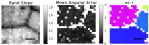
\includegraphics[width=0.6\textwidth]{figurer/astroebsd_output/astroebsd_output.eps}
  \caption{Parts of the indexing output from AstroEBSD for our example data set. The scale bar is \SI{5}{\micro\metre}.}
  \label{fig:astroebsd-output}
\end{figure}

All output data from AstroEBSD is stored in an output .mat file found in the output directory. I've made a script \texttt{astroebsd2mtex.m} \footnote{\texttt{astroebsd2mtex} GitHub repository: \url{https://github.com/hwagit/mtex-snippets/tree/master/astroebsd2mtex}.} to export sample position (x, y), Euler angles, pattern quality, pattern slope, mean angular error, band number and phase per sample position to a .dat file which can be read by the open source and powerful Matlab toolbox MTEX \footnote{MTEX homepage: \url{https://mtex-toolbox.github.io/documentation.html} (visited on 03/14/2019).}. With MTEX you can analyse and model crystallographic textures by means of EBSD or pole figure data. In the same GitHub repository as \texttt{astroebsd2mtex.m} I've added a script showing an example usage of it together with MTEX. The workflow in the script is as follows:

\begin{enumerate}
  \item Import data.
  \item Filter orientations based on mean angular error.
  \item Reconstruct grains, remove smallest grains, reconstruct grains again and finally lightly smooth the grain boundaries.
  \item Lightly smooth orientation data and fill in filtered out orientations.
  \item Plot band slope, mean angular error and inverse pole figure map, all with grain boundaries overlayed.
\end{enumerate}

The results from MTEX is shown in Fig. \ref{fig:mtex-output}.

\begin{figure}[ht]
  \centering
  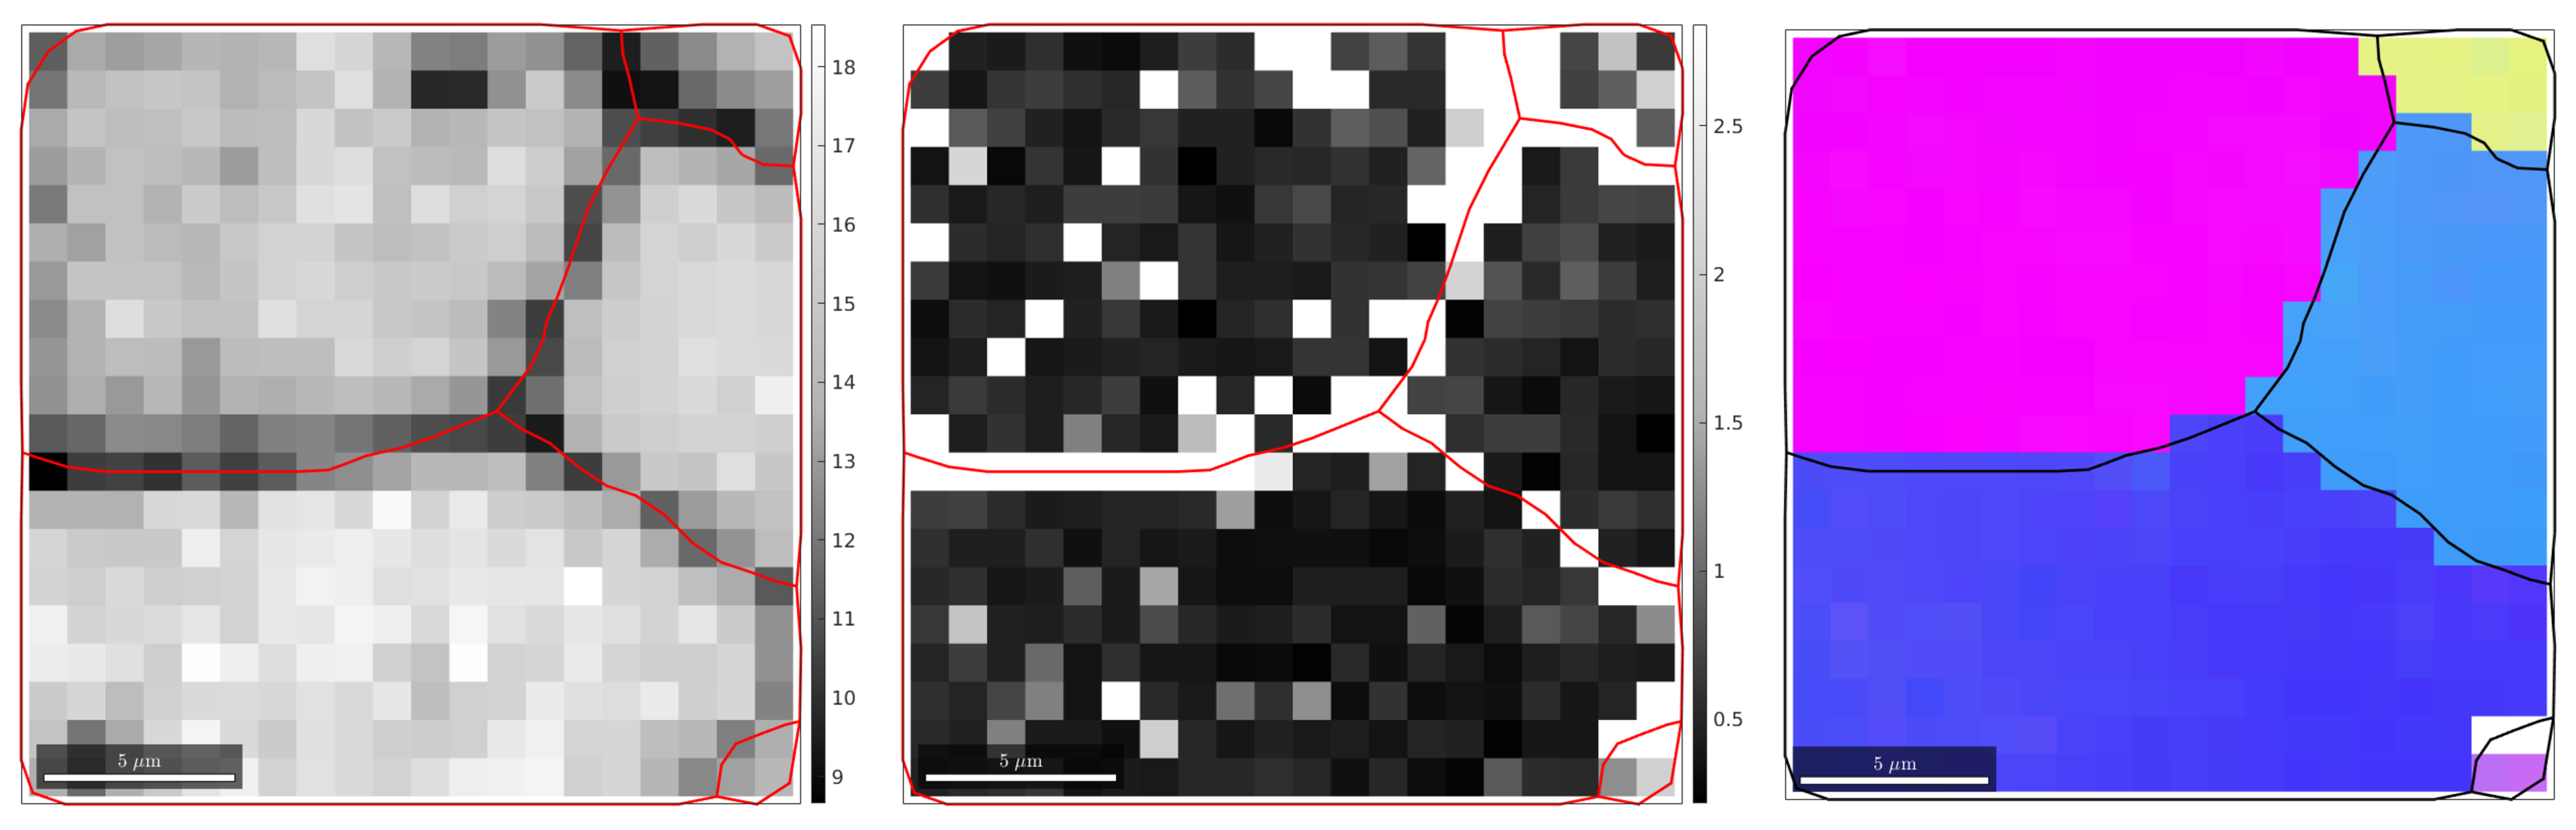
\includegraphics[width=0.5\textwidth]{figurer/mtex_output/mtex_output.eps}
  \caption{Same output from MTEX as from AstroEBSD in Fig. \ref{fig:astroebsd-output}, with grain boundaries overlayed. The orientation data processing is explained in the text above.}
  \label{fig:mtex-output}
\end{figure}

%%%%%%%%%%

\printbibliography

\end{document}
